% \clearpage % NOTE: This one has an impact.
\section{Hyperparameters}
% COULDDO[no time]: Explain the hyperparameters prior to showing any results. (@Leonora)

Hyperparameters are parameters that are not learned from the data,
but adjusted by the user.
%
In order to find the optimal hyperparameters,
the unfolding procedure is repeated for different values of the hyperparameters.

% The hyperparameters which are expected to be mostly independent of others are checked first (see \autoref{sec:hyperparameters:initial_bayesian}).
% Then, the remaining hyperparameters are checked in separate grid searches.

A starting point is determined by Bayesian optimization of the hyperparameters
  (see \autoref{sec:hyperparameters:initial_bayesian}).
Then, individual grid searches are performed for the hyperparameters of interest.
%
In each case, 10-fold cross-validation is utilized to reduce the variance of single data points
  (see \autoref{sec:hyperparameters:cross_validation}).

% ↓ see pp. 46-48 of dsea_mirko
The adaptive step size method of \dseaplus{}
  (see \autoref{sec:dsea:dsea:step_size:adaptive})
is used
because it performs well with all reasonable convergence thresholds.
It eliminates the need to optimize for step size related hyperparameters,
  such as
    exponential vs. multiplicative decay
    or the initial step size,
  apart from the $J$-factor,
    which only has a minor effect on the results,
and provides accurate results after a few iterations \cite{dsea_mirko}.

Since \ac{Adam} maintains separate learning rates for each parameter,
optimization for the learning rate is not essential.
This is verified by the initial Bayesian optimization (\autoref{sec:hyperparameters:initial_bayesian}),
  where the results have no significant correlation with the learning rate.


\subsection{Cross-Validation} \label{sec:hyperparameters:cross_validation}
Cross-validation \cite{cross_validation} is a method to evaluate the performance of a model on unseen data
without having to reserve a part of the data for testing.
%
The data is split into $k$ \emph{folds} of equal size. % NOTE: not to be confused with DSEA's iteration index k
The model is then trained on $k-1$ folds,
and evaluated on the remaining fold.
This is repeated $k$ times,
each time using a different fold for evaluation.
The average of the results is then used as the performance metric.

In this work,
cross-validation is used primarily to get more meaningful performance metrics
for each hyperparameter setting,
  % which would otherwise [be noisy / good by chance / …].
  since individual runs have a high variance.
The number of folds is set to $k = 10$,
  striking a balance between
    the size of the data set,
    the statistical uncertainty,
    and the computational cost.


% “These are the baseline hyperparameters as determined by a Bayesian optimization search.
% Grid searches for individual hyperparameters will show that these are actually optimal.”
% (I hope.)
\subsection{Initial Bayesian Search} \label{sec:hyperparameters:initial_bayesian}
Since a grid search is computationally expensive,
  especially for a large number of hyperparameters,
a Bayesian optimization search \cite{wandb_bayesian} is used to find a good starting point for the grid search.
Contrary to a random search,
the results of previous runs are taken into account
  by building a probabilistic model of the objective function
    (in this case, the Wasserstein distance),
  which allows the search to focus on promising areas of the hyperparameter space.

\begin{figure}
  \centering
  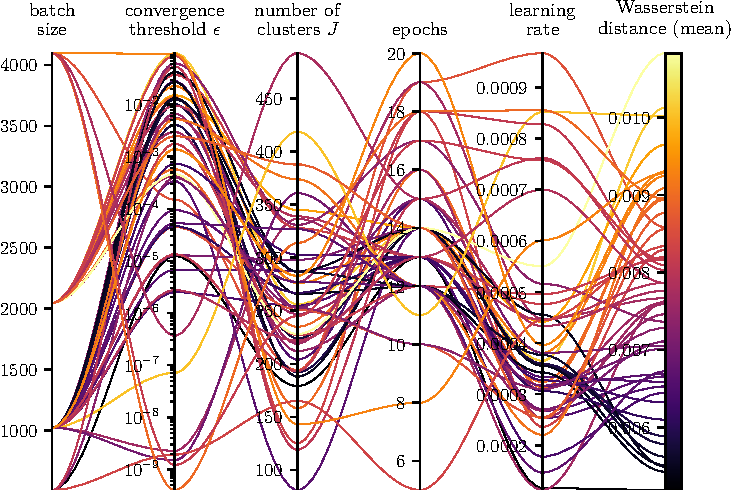
\includegraphics[scale=1]{content/plots/hyperparam/combined_pcplot_full.pdf}
  \caption{
    Parallel coordinates plot of the initial Bayesian hyperparameter search.
    For clarity, only the mean of each 10-fold cross-validation run is shown.
  }
  \label{fig:hyperparameter:bayesian}
\end{figure}

\autoref{fig:hyperparameter:bayesian} shows the results of the Bayesian hyperparameter search.
Based on these results,
the initial hyperparameters are set to the values shown in \autoref{tab:hyperparameters:initial}.

\begin{table}
  \centering
  \begin{tabular}{l r}
    \toprule
    hyperparameter & {value} \\
    \midrule
    % ↓ Analyzed in detail
    batch size & \num{1024} \\
    convergence threshold $\epsilon$ & \num{E-2} \\
    clusters $J$ & \num{250} \\
    epochs & \num{12} \\
    % ↓ Not analyzed further
    learning rate & \num{0.0004} \\
    \bottomrule
  \end{tabular}
  \caption{
    Optimal hyperparameters as determined by a Bayesian optimization search.
  }
  \label{tab:hyperparameters:initial}
\end{table}


\FloatBarrier
\clearpage % NOTE: This one has an impact.
\subsection{Batch Size}
The \emph{batch size} determines the number of events used for each training step.
While larger batch sizes increase the training speed
on optimized hardware,
the performance of the model can be negatively affected \cite{batchsize_kandel}.
% NOTE: not-so-relevant citation

The box plot in \autoref{fig:hyperparameter:batch_size} shows the results of a grid search for the batch size.
% As expected, the performance is worse for larger batch sizes.
A batch size of \num{4096} is chosen as the optimal value,
  not only because it has
    the smallest Wasserstein distance
    and low variance,
  but also because it allows for a faster training time
    compared to smaller values.

\begin{figure}
  \centering
  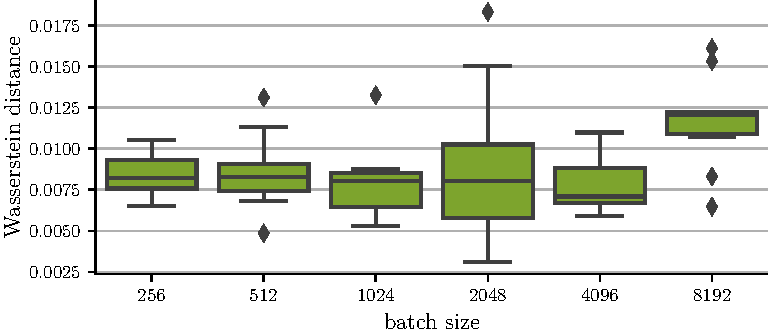
\includegraphics[scale=1]{content/plots/hyperparam/batch_size_vs_wd_boxplot_lessheight.pdf}
  \caption{Box plot of the performance of the model for different batch sizes.
    The performance is measured using the \emph{Wasserstein distance}.
    The box shows the 25th to 75th percentile,
    the center line denotes the median,
    % NOTE: Imprecise. The whiskers extend from the box by up to 1.5x the inter-quartile range (IQR).
    % https://matplotlib.org/stable/api/_as_gen/matplotlib.axes.Axes.boxplot.html
    and the whiskers show the minimum and maximum,
      apart from outliers,
        which are shown as dots.
    A dashed orange line indicates the best median value.
  }
  \label{fig:hyperparameter:batch_size}
\end{figure}


\subsection{Convergence Threshold}
The box plot in \autoref{fig:hyperparameter:epsilon} shows the results of a grid search for the convergence threshold
  (as described in \autoref{sec:dsea:dsea:step_size}).
%
For larger values,
  the performance tends to improve,
  % NOTE: Mirko had better results for smaller values, at least with non-adaptive step sizes.
  until approximately $\epsilon > \num{0.05}$.
This is because a high convergence threshold can be thought of as
  a form of \emph{implicit} regularization, % @Mirko
    analogous to early stopping,
  contrary to \emph{explicit} regularization,
    as described in \autoref{sec:dsea:deconvolution_problem:regularization}.
Selecting even higher values of $\epsilon$
  (not shown in the plot)
stops \dsea{} after the first iteration,
  which results in particularly poor performance.
$\epsilon = \num{0.025}$ is chosen as the optimal value.


\begin{figure}
  \centering
  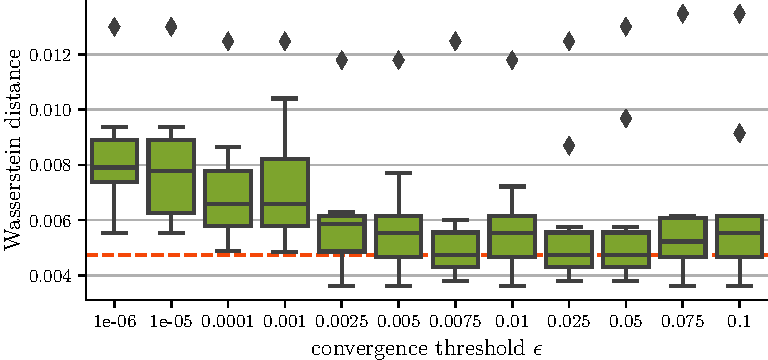
\includegraphics[width=\textwidth]{content/plots/hyperparam/epsilon_vs_wd_boxplot_lessheight.pdf}
  \caption{
    Box plot of the Wasserstein distance for different convergence thresholds.
    Note that the abscissa is not uniformly spaced.
  }
  \label{fig:hyperparameter:epsilon}
\end{figure}


\subsection{Number of Clusters}
The adaptive step size function,
  which has been explained in \autoref{sec:dsea:dsea:step_size:adaptive}, % NOTE: already linked in the previous subsection
internally relies on clustering the data into $J$ clusters.
The number of clusters $J$ is therefore a hyperparameter of the algorithm.
%
Large values of $J$ have previously been shown to lead to slightly better results \cite{dsea_mirko}.
\autoref{fig:hyperparameter:J} confirms this,
although the median does not decrease monotonically with $J$.
The optimal value is \num{200},
which has a slightly better performance than \num{500}.

\begin{figure}
  \centering
  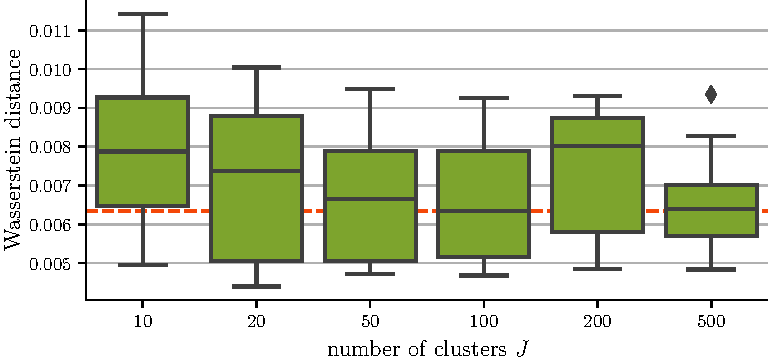
\includegraphics[scale=1]{content/plots/hyperparam/J_vs_wd_boxplot_lessheight.pdf}
  \caption{Box plot of the Wasserstein distance for different numbers of clusters.}
  \label{fig:hyperparameter:J}
\end{figure}


\subsection{Number of Epochs}
While a higher number of epochs typically increases the model's performance on the training data,
it also increases the risk of overfitting.
%
\autoref{fig:hyperparameter:epochs} visualizes a hyperparameter search for the number of epochs per \dsea{} iteration.
The results show that the model's performance on the training data is best for \num{12} epochs.
\autoref{fig:hyperparameter:num_epochs_vs_wd_boxplot} shows that
the accuracy is not negatively affected by a higher number of epochs,
  indicating that the model is not overfitting.

\begin{figure}
  \centering
  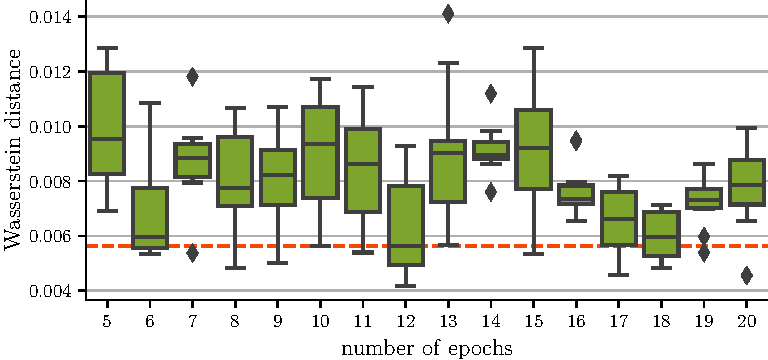
\includegraphics[width=\textwidth]{content/plots/hyperparam/num_epochs_vs_wd_boxplot_lessheight.pdf}
  \caption{Box plot of the Wasserstein distance for different epoch counts.}
  \label{fig:hyperparameter:epochs}
\end{figure}
